\documentclass[smallextended]{svjour3}


% \documentclass[12pt,a4paper]{article}
\RequirePackage{tikz}
% \documentclass[sn-apacite,xelatex]{sn-jnl}
% \usepackage{program}
% \catcode`\|=12\relax

\usepackage[margin=1in]{geometry}
\usepackage[toc]{appendix}
% \usepackage{natbib}
\usepackage[backend=biber, style=apa, sortcites=false, uniquelist=false,natbib=true,doi=false,isbn=false,url=false,eprint=false,pagetracker, ibidtracker=constrict]{biblatex}
\DeclareSourcemap{
  \maps{
    \map{
      \step[fieldset=entrysubtype, null]
      \step[fieldset=address, null]
      \step[fieldset=location, null]
    }
  }
}

\addbibresource{references.bib}

% \usepackage{authblk}
% \usepackage[hyperref]{acl2020}
\usepackage[colorlinks=true,citecolor=blue]{hyperref}
% \usepackage{times}
\usepackage{latexsym}
\usepackage{graphicx}
% \usepackage{subcaption}
% \usepackage{float}

\usepackage{tikz}
% \usepackage{tikzscale}
\usepackage{pgfplots}
\usetikzlibrary{shapes,positioning,calc}

\usepackage{longtable}
\usepackage{multirow}
\usepackage{multicol}

\usepackage{amsmath}
\usepackage{amssymb}
% \usepackage{bbm}
\usepackage{dsfont}
% \usepackage[utf8x]{inputenc}
\usepackage{textcomp}
\usepackage{textgreek}
\usepackage[french,english]{babel}
\usepackage{latexsym}
\usepackage{url}  %Required
\usepackage{graphicx}  %Required
\frenchspacing  %Required
\usepackage{url}
\usepackage{booktabs}
\usepackage{array}
\renewcommand{\UrlFont}{\ttfamily\small}

\usepackage[acronym,nomain,nonumberlist]{glossaries}
\makeglossaries
\renewcommand*{\glsgroupskip}{}


\newacronym{doe}{DoE}{Department of Energy}
\newacronym{nsf}{NSF}{National Science Foundation}
\newacronym{oatd}{OATD}{Open Access Theses and Dissertations}
\newacronym{orcid}{ORCID}{Open Researcher and Contributor ID}

\newacronym{lep}{LEP}{Large Electron Positron Collider}
\newacronym{ssc}{SSC}{Superconducting Super Collider}
\newacronym{lhc}{LHC}{Large Hadron Collider}
\newacronym{fcc}{FCC}{Future Circular Collider}
\newacronym{eht}{EHT}{Event Horizon Telescope}
\newacronym{wos}{WoS}{Web of Science}

\newacronym{desy}{DESY}{\textit{Deutsches Elektronen-Synchrotron}}
\newacronym{slac}{SLAC}{Stanford Linear Accelerator Center}
\newacronym{cern}{CERN}{Conseil Européen de Recherche Nucléaire}

\newacronym{mssm}{MSSM}{Minimal Supersymmetric Standard Model}
\newacronym{pmssm}{pMSSM}{Phenomenological Minimal Supersymmetric Standard Model}
\newacronym{cmssm}{cMSSM}{constrainted Minimal Supersymmetric Standard Model}

\newacronym{aip}{AIP}{American Institute of Physics}
\newacronym{pacs}{PACS}{Physics and Astronomy Classification Scheme\textregistered}

\newacronym{sm}{SM}{Standard Model of Particle Physics}
\newacronym{ms}{MS}{Modèle Standard de la physique des particules}
\newacronym{hep}{HEP}{High-Energy Physics}
\newacronym{bsm}{BSM}{Beyond the Standard Model}

\newacronym{wimp}{WIMPs}{Weakly Interacting Massive Particles}

\newacronym{hi}{HI}{Historical Institutionalism}
\newacronym{cha}{CHA}{Comparative Historical Analysis}


%%% HELPER CODE FOR DEALING WITH EXTERNAL REFERENCES
\usepackage{xr}
\makeatletter
\newcommand*{\addFileDependency}[1]{
  \typeout{(#1)}
  \@addtofilelist{#1}
  \IfFileExists{#1}{}{\typeout{No file #1.}}
}
\makeatother

\newcommand*{\myexternaldocument}[1]{
    \externaldocument{#1}
    \addFileDependency{#1.tex}
    \addFileDependency{#1.aux}
}
%%% END HELPER CODE



\myexternaldocument{main}
\usepackage{prettyref}
\newrefformat{fig}{\ref{#1}}
\newrefformat{table}{\ref{#1}}
\newrefformat{appendix}{\ref{#1}}
\newrefformat{sec}{\ref{#1}}
\newrefformat{section}{\ref{#1}}

\renewcommand{\thefigure}{S\arabic{figure}}
\renewcommand{\thetable}{S\arabic{table}}
\renewcommand{\thesection}{S\arabic{section}}


\title{Supplementary materials for ``How research programs come apart''}

\author{Lucas Gautheron \and Elisa Omodei}

\date{}

\journalname{Quantitative Science Studies}

\begin{document}

\maketitle

% \appendix

% \section{Appendices}
\label{section:appendix}

\section{Data collection}
\label{appendix:collection}

Our goal was to collect the whole HEP literature from 1980 to 2020 from the public Inspire HEP API \citep{InspireAPI}. For that, we collected metadata for all articles through automated search requests, category per category, and year per year. This strategy was intended to abide with the limitations of the API, in terms of matching entries per search request. However, it appeared that many articles in years 1990 to 1995 were not categorized, and therefore our collection strategy missed many HEP articles from this period. In order to recover these articles, we gathered all articles that were referenced in publications collected through the first batch but which were missing. This methods fails to recover articles that were not cited in any article from the first batch. More importantly, 
the lack of categories means that selecting all HEP papers during the problematic time period will require unlabeled articles to be manually or automatically classified. Although there are ways to circumvent these issues and to assess their potential implications, we have decided to narrow down several analyses to years 2001 onwards in the present work.

% \section{Predicting categories}

\section{\label{appendix:stability}Text-classifier performance stability}

The categories (\texttt{Theory-HEP}, \texttt{Phenomenology-HEP} and \texttt{Experiment-HEP}) that we trained our classifier (\ref{section:method_subcultures}) to predict have been assigned in different ways in the Inspire HEP database. Although a majority were categorized based on arXiv's classification system, some papers were not, especially those published before arXix was introduced (in the early 1990s). It might seem unclear whether these classification procedures are consistent and revealing of distinct underlying cultures. In order to demonstrate that it is the case, in Figure \prettyref{fig:stability}, we show that the performance of the text-classifier is nonetheless roughly stable throughout the period considered (1980--2020). To this end, we subdivide this time-range in bins of five years and perform k-fold cross-validation using each five year bin for the validation set (and the papers from the other bins for the training set). Accuracy remains high and approximately stable over the years 1980 to 2020; therefore, these various classification procedures, and the underlying identity of each of these subcultures, must be rather consistent over this period.

\begin{figure}
    \centering
    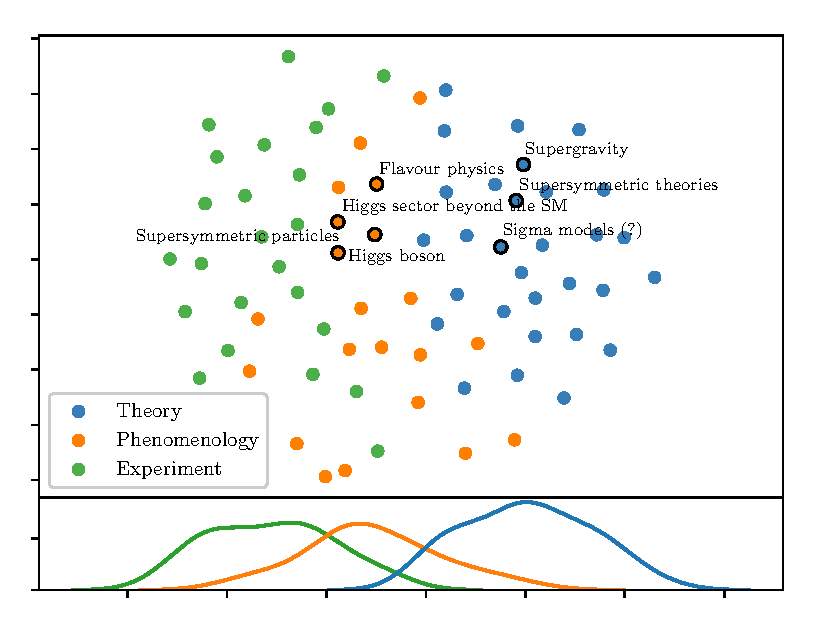
\includegraphics{Fig8.eps}
    \caption{Accuracy of the text-classifier from Section \ref{section:method_subcultures} as a function of the papers' years of publication. Error-bars represent the 95\% confidence interval. Dashed lines show the accuracy of the baseline model (which may vary only due to variations in the frequency of each category, since the baseline model always predicts the most common class). The accuracy is roughly constant across time for each of the three categories, despite significant variations in the frequency of each class.}
    \label{fig:stability}
\end{figure}



\section{Topic model}


\subsection{\label{appendix:data_selection}Data and vocabulary selection}

The model is trained on $N=120,000$ articles randomly sampled from those in the 1980-2020 period that belong to any of the categories \texttt{Theory-HEP}, \texttt{Phenomenology-HEP}, \texttt{Experiment-HEP}, and \texttt{Lattice}. Titles and abstracts of each papers are concatenated in order to maximize the textual content used for training. Very short texts (less than 100 characters) are removed.

Before applying the model, we performed a number of pre-processing steps on the abstracts with the goal of maximizing the amount of useful information in the training data. This procedure, largely inspired from \citealt{omodei_tel-01097702} and implemented with the use of the NLTK library \citep{nltk}, is as follows:

\begin{itemize}
    \item Tokens (words separated by punctuation or spaces) are extracted from the text and transformed to lower-case.
    \item All single nouns and adjectives are retrieved from these tokens.
    \item We also retrieve all n-grams that match specific syntactic patterns (e.g. ``adjective+noun+noun'', such as ``supersymmetric standard model'', ``effective field theory'').
    \item Single words are lemmatized, i.e. they are normalized to their root (e.g. ``symmetries'' becomes ``symmetry'').
    \item Words and expressions that occur less than 20 times are removed.
\end{itemize}

First, these steps allow us to reduce noise by removing words that convey little to no information about the topics of the articles (such as stop words). Second, extracting n-grams that matching certain syntactic patterns allows us to preserve some information about the relative position of words within the abstracts -- which CTM do not do otherwise -- while taking advantage of our prior knowledge of the documents' language. For instance, the word ``dark'' may convey different meanings depending on whether it occurs immediately before the word ``matter'', or, alternatively, ``energy''; similarly, the occurrence of the expression ``dark matter'' in a text conveys more information than the simultaneous occurrence of ``dark'' and ``matter'' without more knowledge about their relative position.

As a result of this procedure, the vocabulary contains $V=$ 18,658 ``words'', with 58 words per article on average.

\subsection{\label{appendix:hyper_parameter}Hyper-parameters}

The implementation of the CTM by Tomotopy \citep{tomotopy} has three hyper-parameters: the amount of topics $k$, an $\vec{\alpha}$ parameter that controls the sparsity of the document-topic distribution ($\theta_{d,i}$), and a $\vec{\eta}$ parameter that controls the sparsity of the topic-word distribution (the vocabulary associated to each topic).
For choosing the amount of topics $k$, we considered three values that seemed acceptable in terms of interpretability and compliance with the values from the literature: 50, 75 and 100.
We assumed $\vec{\alpha}$ and $\vec{\eta}$ to be symmetric, i.e. $\alpha_1 = \alpha_k = \alpha$ and $\eta_1 = ... = \eta_V = \eta$\footnote{This is common in the literature, but this choice is disputable, cf. \citealt{Wallach2009}. One implication of symmetric priors is that topics must have comparable probabilities. This also has an impact on the meaning of topics.}. We considered  $\alpha \in \{10^{-2},10^{-1},1\}$ and $\eta \in \{10^{-3},10^{-2},10^{-1}\}$, according to values encountered in the literature.
We then trained the model for each triplet of $k$, $\alpha$ and $\eta$ among the candidate values. We rejected all triplets that led to significant overfitting, by comparing the perplexity\footnote{Perplexity is the exponential of the average log-likelihood per word, cf. \citealt{Blei2003}. It measures the improbability of a corpus according to a given model.} obtained for the training corpus and that obtained by applying the trained model to a validation set of abstracts unseen during training.
Although \citet{Chang2009} have shown that perplexity could be negatively correlated to human judgments about the interpretability of the topics recovered by topic models, we believe it is a suitable metric to discard models that fail to capture meaningful regularities in the data, which is the case of models that show overfitting. Among the remaining models, we then selected the two models with the highest normalized pointwise mutual information coherence, a coherence metric frequently used to assess the consistency of topic models \citep{hoyle2021is}. Topic coherence metrics in general, as stressed by \citeauthor{hoyle2021is}, are not very strongly correlated with human judgments about the quality of a model; however, we believe they may be useful to discard certain models in order to limit the amount of those that should be inspected manually (since manual inspection is time-consuming and quite subjective). We finally inspect manually the two models with the highest coherence measure, and choose the one with $k=75$, $\alpha=0.1$ and $\eta=0.001$. Our preference for this model stemmed from the fact that it contained more topics than the other remaining model, and that these more numerous topics seemed reasonably consistent.

\subsection{Validation}
\label{appendix:validation}

Since the model infers document-topic distributions and topic-word distributions, we would like to assess the validity of these metrics, i.e. ``their ability to measure what they purportedly measure'' \citep[p.~3240]{Bannigan2009}. In order to simultaneously assess both measures, we designed the following protocol. First, we derived the \gls{pacs} categories $c$ that were the most correlated to each topic $z$ (this approach is in a sense comparable to that employed in \citealt{Griffiths2004}, who extracted the topics that were more strongly associated with PNAS categories). For that, we listed the categories $c$ that maximize the pointwise mutual information with each topic $z$ according to:

\begin{equation}
    \label{eq:pmi_expression}
    \mathrm{pmi}(z,c) = \log \dfrac{p(z|c)}{p(z)}% = \log \left( \dfrac{\displaystyle\sum_{d \in c} \theta_{d,z}}{\displaystyle\sum_{d} \theta_{d,z}} \times \dfrac{D}{D_c}\right)
\end{equation}

Where $p(z)$ is the marginal probability of the topic $z$, and $p(z|c)$ the probability that a word in a document belongs to a topic $z$ given that the document was assigned the PACS category $c$. Thefore, $\mathrm{pmi}(z,c)$ measures the increase in probability of a given topic provided that a PACS category is present. The 5 categories most correlated to each topic are given in table \prettyref{table:full_topics_pacs_pmi}, which helped inform our choice for each tpic label, in complement to their top-words.

Then, we submitted the lists of PACS categories thus constitued to a human task derived from the methodology of \citet{Bennett2021}, as follows:

\begin{enumerate}
    \item We draw at random a topic $z_1$ with a probability equal to its marginal probability 
    \item We draw at random 5 PACS categories $c_1,...,c_5$ among the 10 most correlated to $z_1$, as described above.
    \item Then, we do any of the following, with equal probability $1/2$:
    \begin{enumerate}
        \item We draw at random another topic $z_2\neq z_1$ with probability $p(z_2)\over 1-p(z_1)$, and we pick at random 5 PACS categories $c_6,...,c_{10}$ among those most correlated with it.
        \item Alternatively, we draw  $c_6,...,c_{10}$ from the 5 remaining PACS categories most associated to $z_1$
    \end{enumerate}
    \item We submit $c_1, ..., c_5$ and $c_6, ..., c_{10}$ to an expert unaware of the model. The expert is asked to guess whether the two lists of 5 categories were drawn from one and same general topic, or whether they were drawn from two separate topics.
    \item The procedure is repeated a certain amount of times. The final score is the fraction of correct responses.
\end{enumerate}

The rationale for this method is that good scores should only be achievable provided the topics are rather coherent, and that the document-topic distributions $\theta_{d,i}$ are reasonably accurate. The final average score is 0.74 for 100 guesses from two HEP PhD students, which is significantly better than a random baseline (0.5). This shows that, to some extent, the topic distributions derived for each article correlate with \gls{pacs} categories that are rather coherent with each other.

\subsection{\label{appendix:topics}Topics}

% \clearpage
% \onecolumn

\fontsize{6}{7}\selectfont\begin{longtable}[H]{p{0.2\textwidth}|p{0.8\textwidth}}
\caption{Most frequent terms for each topic.}
\label{table:top_words}\\ \midrule
\toprule
{} &                                                                                                                                                                                  Most frequent expressions \\ \midrule
Topic (context)                                       &                                                                                                                                                                                                            \\ \midrule
\midrule
\endfirsthead
\caption[]{Most frequent terms for each topic.} \\ \midrule
\toprule
{} &                                                                                                                                                                                  Most frequent expressions \\ \midrule
Topic (context)                                       &                                                                                                                                                                                                            \\ \midrule
\midrule
\endhead
\midrule
\multicolumn{2}{r}{{Continued on next page}} \\ \midrule
\midrule
\endfoot

\bottomrule
\endlastfoot
Algorithms and calculation techniques                 &                                                               simulation, carlo, monte, lattice, method, correlation, distribution, cluster, generator, statistical, study, function, scaling, size, event \\ \midrule
Amplitude of processes in colliders                   &                                                     amplitude, contribution, state, interaction, resonance, final, final state, process, exchange, reaction, tree, scattering, double, polarization, level \\ \midrule
Amplitudes and Feynman Diagram                        &                                                             amplitude, function, loop, limit, pole, conformal, relation, integral, diagram, correlation, scattering, analytic, block, correlators, feynman \\ \midrule
Analyses and measurements from colliders              &                                                                         data, measurement, event, result, detector, experiment, gev, algorithm, analysis, muon, experimental, energy, precision, fit, beam \\ \midrule
Annihilation and scattering cross-sections            &                                             section, cross, annihilation, photon, energy, scattering, gev, production, total, elastic, process, pair, total cross section, total cross, elastic scattering \\ \midrule
Astrophysics                                          &                                              star, wave, nuclear, matter, neutron, collision, gravitational waves, energy, nuclear matter, flow, density, gravitational, relativistic, heavy-ion, equation \\ \midrule
Black holes                                           &                                black, hole, black hole, black holes, horizon, entropy, extremal, radiation, schwarzschild, thermodynamics, black hole solutions, black hole entropy, hawking, charge, kerr \\ \midrule
Boundary conditions/non-locality                      &                                              boundary, condition, boundary conditions, state, tensor, entropy, entanglement, distance, case, surface, general, correlation, boundary condition, term, phys \\ \midrule
CP violating processes                                &                                                        cp, asymmetry, violation, parameter, $b^0$, bound, direct cp, direct, mixing, penguin, decay, constraint, experimental, direct cp violation, effect \\ \midrule
Conformal Field Theory                                &           conformal, string, algebra, theory, conformal field, conformal field theory, central, central charge, conformal field theories, charge, operator, open, superconformal, virasoro, representation \\ \midrule
Cosmological sources                                  &                                                       cosmic, spectrum, scale, energy, ray, universe, radiation, gravitational, cosmological, power, observation, cmb, background, cosmic ray, cosmic rays \\ \midrule
Cosmology and gravity                                 &                                                      cosmological, gravity, constant, axion, scale, lorentz, universe, cosmological constant, violation, problem, quantum, vacuum, cosmology, time, planck \\ \midrule
Cross-sections in colliders                           &                                                                             production, section, cross, collision, energy, lhc, rapidity, process, pair, pp, inclusive, differential, fusion, nuclear, gev \\ \midrule
Dark matter (particles and direct searches)           &                                                         dark matter, matter, dark, dm, particle, detection, direct detection, direct, wimp, relic, relic density, density, annihilation, search, candidate \\ \midrule
Dark matter in the universe                           &                                                                 dark, matter, dark matter, dark energy, model, abundance, energy, sector, constraint, density, candidate, galaxy, universe, cold, scenario \\ \midrule
Decay measurements                                    &                                                                                         decay, state, $d$, meson, stat, syst, $+/-$, $+-$, fraction, final, final state, width, ratio, $pi+$, final states \\ \midrule
Detectors                                             &                                                               detector, experiment, physic, beam, high, crystal, nuclear, liquid, performance, precision, resolution, high energy, search, target, chamber \\ \midrule
Double-beta decay                                     &                                                                 mass, baryon, decay, scalar, beta, double beta decay, double, double beta, scale, light, neutrinoless, effective, glueball, gev, hierarchy \\ \midrule
Early-universe and other cosmological data            &                                                                      constraint, big bang, big, galactic, signal, cosmic microwave, background, axion, bound, galaxy, bang, microwave, halo, detection, dm \\ \midrule
Effective Field Theory                                &  field, effective, theory, effective field theory, effective field, noncommutative, action, effective action, scalar, scalar field, potential, effective theory, effective potential, eft, non-commutative \\ \midrule
Electromagnetism                                      &                               magnetic, field, particle, magnetic field, electric, relativistic, electromagnetic, effect, plasma, moment, energy, medium, magnetic fields, external, electromagnetic field \\ \midrule
Events in colliders (kinematics?)                     &                                                               production, collision, jet, tev, lhc, collider, event, transverse, large hadron collider, energy, large hadron, hadron, pair, pp, luminosity \\ \midrule
Events in colliders (signatures?)                     &                                                                         jet, event, lhc, tev, production, cm, pair, atlas, final state, final, collision, data, luminosity, channel, large hadron collider \\ \midrule
Experimental investigation of the leptonic sector     &                                                                           decay, search, data, limit, gamma, collider, muon, gev, measurement, signal, experiment, detector, magnetic moment, event, upper \\ \midrule
Experimental jargon                                   &                                                                                 result, mass, effect, large, parameter, energy, value, analysis, small, order, region, current, due, contribution, present \\ \midrule
Experiments on light                                  &                                                                                              photon, electron, particle, experiment, mi, laser, compton, optical, mo, beam, light, atom, year, math, pulse \\ \midrule
Field theory and gravity                              &                                              scalar, field, scalar field, mode, gravity, massive, scalar fields, gravitational, potential, massless, perturbation, geodesic, background, metric, spacetime \\ \midrule
Flavor mixing                                         &                                                                         cp, violation, asymmetry, mixing, matrix, lepton, cp violation, flavor, standard model, model, quark, phase, standard, angle, mass \\ \midrule
Flavour physics                                       &                                                                                 mass, lepton, bound, flavour, flavor, decay, neutrino, heavy, scale, generation, violation, light, quark, coupling, number \\ \midrule
Form factors                                          &                                  factor, form, nucleon, electromagnetic, pion, electromagnetic form, electromagnetic form factors, momentum, form factors, result, ratio, $^2$, transfer, nn, form-factors \\ \midrule
Gauge Theory                                          &                                              gauge, theory, action, invariance, field, lorentz, transformation, invariant, brst, yang-mills, symmetry, effective action, lattice gauge, massive, covariant \\ \midrule
Gauge symmetry breaking/GUTs                          &                                                                symmetry, gauge, su, model, group, theory, breaking, anomaly, fermion, spontaneous, unification, representation, discrete, symmetric, grand \\ \midrule
Gravitons and extra-dimensions                        &                                        gravity, dimension, scalar, extra, field, constant, brane, cosmological, massive, cosmological constant, extra dimensions, scalar field, bulk, graviton, derivative \\ \midrule
Hadronic zoo                                          &                                                                                            state, resonance, $d$, gev, mev, $b$, channel, $e^+e^-$, charmonium, narrow, $b$, molecule, s1, reaction, $e^+$ \\ \midrule
Heavy quarks and ions                                 &                                                     quark, heavy, hadron, distribution, collision, production, gluon, hadronic, qcd, heavy quark, heavy ion, charm, correlation, ion, heavy ion collisions \\ \midrule
Higgs boson                                           &                                                                        higgs, boson, model, standard model, mass, standard, coupling, gauge, sector, sm, higgs mass, doublet, higgs boson, neutral, scalar \\ \midrule
Higgs sector beyond the SM                            &                              higgs, model, standard model, standard, boson, electroweak, supersymmetric, lhc, minimal, supersymmetric standard model, collider, tev, mass, scalar, supersymmetric standard \\ \midrule
High-energy source fluxes                             &                                                                  energy, flux, source, high energy, spectrum, high, event, signal, emission, time, radiation, solar, information, gravitational wave, such \\ \midrule
Holographic Principle and dualities                   &                                conformal, dual, holographic, boundary, entropy, cft, entanglement, ad, bulk, defect, theory, conformal field, correspondence, conformal field theory, entanglement entropy \\ \midrule
Inflation                                             &                                     inflation, perturbation, universe, inflationary, field, scalar, cosmological, inflaton, cosmology, potential, scalar field, initial, evolution, fluctuation, curvature \\ \midrule
Lattice calculation techniques                        &                                                                      operator, lattice, matrix, fermion, loop, wilson, theory, element, gauge, function, action, calculation, continuum, expansion, method \\ \midrule
Lepton/Meson decay                                    &                                                               decay, branching, ratio, semileptonic, meson, fraction, asymmetry, mode, measurement, rate, br, nu, semileptonic decays, inclusive, lifetime \\ \midrule
Lie algebra                                           &                                                          algebra, space, integral, representation, function, group, operator, invariant, form, path, transformation, lie, differential, product, partition \\ \midrule
Loops and higher order expansions in Feynman Diagrams &                                    correction, order, one-loop, term, contribution, radiative corrections, approximation, qed, calculation, loop, radiative, logarithmic, effective, expansion, expression \\ \midrule
M-theory and theories of everything                   &                                                                  theory, gauge, duality, supergravity, string, dual, action, dimensional, type, background, m-theory, reduction, dimension, abelian, field \\ \midrule
Matter in Yang-Mills theories                         &                                                                                       su, symmetry, fermion, gauge, chiral, mass, model, breaking, coupling, boson, flavor, color, composite, quark, dirac \\ \midrule
Measurements and analysis of colliders data           &                                                data, measurement, uncertainty, experiment, analysis, experimental, fit, determination, systematic, first, theoretical, error, parameter, detector, current \\ \midrule
Meson phenomenology                                   &                                                                                meson, state, resonance, vector, decay, mass, width, mev, pseudoscalar, pion, amplitude, experimental, channel, quark, wave \\ \midrule
Neutrino physics                                      &                 neutrino, oscillation, mass, experiment, majorana, neutrino mass, right-handed, neutrino oscillations, neutrino oscillation, flavor, interaction, supernova, antineutrino, seesaw, sterile \\ \midrule
Non-abelian theories                                  &                                                                  gauge, field, spin, topological, theory, chern-simons, higher spin, abelian, vortex, non-abelian, gauge field, dirac, term, hall, fermion \\ \midrule
Partons distributions                                 &                                           qcd, distribution, parton, next-to-leading order, order, function, nlo, gluon, jet, next-to-leading, correction, transverse, momentum, calculation, perturbative \\ \midrule
Perturbative QCD                                      &                           qcd, perturbative, factorization, anomalous, order, contribution, result, function, approach, perturbative qcd, calculation, anomalous dimension, coefficient, kernel, expansion \\ \midrule
Phenomenological jargon                               &                                                                                   state, new, interaction, coupling, physic, strong, problem, particle, theory, recent, such, bound, model, approach, role \\ \midrule
QCD calculation techniques                            &                                                             propagator, expansion, lattice, gluon, effective, finite, loop, theory, potential, qcd, numerical, gauge, perturbative, method, regularization \\ \midrule
Quantum Chromodynamics (QCD)                          &                                                                          rule, sum, qcd, wall, domain, qcd sum rules, viscosity, qcd sum, quark, heavy, shear viscosity, shear, vacuum, condensate, bubble \\ \midrule
Quantum Field Theory                                  &                                 theory, field, quantum, equation, solution, classical, dimension, quantum field, class, quantum field theory, problem, space-time, dimensional, two-dimensional, arbitrary \\ \midrule
Quantum Systems and Equations of motion               &                                                                     equation, hamiltonian, constraint, system, term, formalism, charge, monopole, dirac, solution, first, second, kinetic, nonlinear, part \\ \midrule
Quantum systems and thermodynamics                    &                                                                             system, energy, time, quantum, state, fluctuation, density, gas, dynamic, thermal, temperature, phase, casimir, force, surface \\ \midrule
Renormalization                                       &                                                                             renormalization, group, flow, point, coupling, scale, fixed, uv, rg, ir, cutoff, infrared, fixed point, effective, ultraviolet \\ \midrule
Scattering of composite particles                     &                                                           scattering, function, data, proton, structure, nucleon, inelastic, distribution, moment, deep, dipole, $q^2$, inelastic scattering, hera, target \\ \midrule
Search for BSM physics                                &                                                                    physic, new, new physics, standard model, experiment, standard, neutral, search, tau, measurement, current, decay, future, lepton, rare \\ \midrule
Sigma models (?)                                      &                                                                model, symmetry, supersymmetric, supersymmetry, sigma, term, integrable, lagrangian, algebra, su, group, chiral, deformation, fermionic, sl \\ \midrule
Solar neutrinos                                       &                 neutrino, oscillation, solar, mixing, solar neutrino, angle, atmospheric, neutrino mass, sterile, atmospheric neutrino, experiment, hierarchy, sterile neutrinos, matrix, sterile neutrino \\ \midrule
Space-time geometry and gravity                       &                                                                 solution, gravity, spacetime, metric, gravitational, ad, geometry, space, flat, curvature, sitter, singularity, general, dilaton, einstein \\ \midrule
Spin/angular momentum/polarization                    &                                                momentum, polarization, asymmetry, angular, spin, distribution, angular momentum, polarized, reaction, transverse, cross, section, beam, production, photon \\ \midrule
States of matter                                      &                                      phase, transition, critical, temperature, point, holographic, spectral, order, exponent, behavior, imaginary, critical point, finite temperature, finite, first order \\ \midrule
String theory                                         &                                                                       string, solution, charge, soliton, branes, configuration, topological, type, monopoles, open, flux, bps, tachyon, background, vortex \\ \midrule
Supergravity                                          &                                                       supergravity, modulus, manifold, type, space, calabi-yau, supersymmetric, geometry, supersymmetry, moduli space, topological, bps, class, curve, iib \\ \midrule
Supersymmetric particles                              &                                                                                  mass, susy, parameter, soft, neutralino, space, scale, mssm, squark, region, scenario, constraint, gluino, gaugino, large \\ \midrule
Supersymmetric theories                               &                                                        theory, gauge, supersymmetric, yang-mills, supersymmetry, anomaly, supergravity, duality, chiral, $n=4$, super, $n=2$, super yang-mills, branch, su \\ \midrule
Symétrie chirale                                      &                                  chiral, quark, qcd, lattice, chiral symmetry, mass, chiral perturbation theory, chiral perturbation, pion, condensate, baryon, transition, perturbation, flavor, symmetry \\ \midrule
Theoretical jargon                                    &                                                                              model, case, structure, limit, new, term, function, such, number, different, method, particular, property, spectrum, approach \\ \midrule
Thermodynamics                                        &                                          phase, temperature, transition, potential, density, chemical, finite, finite temperature, matter, chemical potential, critical, high, thermal, order, first order \\ \midrule
Top quark                                             &                                                       quark, top, top quark, mass, decay, bound, standard model, top quark mass, coupling, new physics, lepton, top quarks, standard, chiral quark, physic \\ \midrule
Topology                                              &                                                                space, dimension, modulus, string, bundle, manifold, vacuum, extra, moduli space, heterotic, torus, instanton, singularity, compact, theory \\ \midrule
\end{longtable}
\normalsize
\fontsize{6}{7}\selectfont\begin{longtable}[H]{p{0.25\textwidth}|p{0.6\textwidth}|p{0.15\textwidth}}
\caption{PACS categories most correlated to the topics derived with the unsupervised model. Correlation is measured as the mutual pointwise information (pmi).}
\label{table:full_topics_pacs_pmi}\\
\toprule
                                        &                    &   pmi \\
topic & PACS category &       \\
\midrule
\endfirsthead
\caption[]{PACS categories most correlated to the topics derived with the unsupervised model. Correlation is measured as the mutual pointwise information (pmi).} \\
\toprule
                                        &                    &   pmi \\
topic & PACS category &       \\
\midrule
\endhead
\midrule
\multicolumn{3}{r}{{Continued on next page}} \\
\midrule
\endfoot

\bottomrule
\endlastfoot
\multirow{5}{*}{\begin{tabular}{l}Algorithms and\\ calculation\\ techniques\end{tabular}} & Lattice theory and statistics &  1.39 \\
                                        & Lattice gauge theory &  1.17 \\
                                        & Lattice QCD calculations &  1.12 \\
                                        & Particle correlations and fluctuations &  0.99 \\
                                        & Inelastic scattering: many-particle final states &  0.80 \\
\cline{1-3}
\multirow{5}{*}{\begin{tabular}{l}Amplitude of\\ scattering\\ processes\end{tabular}} & Baryon resonances (S=C=B=0) &  1.13 \\
                                        & Pion-baryon interactions &  1.10 \\
                                        & Meson-meson interactions &  1.03 \\
                                        & Nucleon-nucleon interactions &  0.93 \\
                                        & Dispersion relations &  0.92 \\
\cline{1-3}
\multirow{5}{*}{\begin{tabular}{l}Amplitudes and\\ Feynman Diagram\end{tabular}} & Analytic properties of S matrix &  1.66 \\
                                        & Properties of perturbation theory &  1.57 \\
                                        & General properties of perturbation theory &  1.39 \\
                                        & Dispersion relations &  1.04 \\
                                        & Lattice theory and statistics &  0.86 \\
\cline{1-3}
\multirow{5}{*}{\begin{tabular}{l}Analyses and\\ measurements\\ from colliders\end{tabular}} & Neutrino-induced reactions &  0.96 \\
                                        & Muons &  0.89 \\
                                        & Neutrino, muon, pion, and other elementary particle detectors; cosmic ray detectors &  0.81 \\
                                        & Pion-baryon interactions &  0.79 \\
                                        & Meson production &  0.77 \\
\cline{1-3}
\multirow{5}{*}{\begin{tabular}{l}Annihilation\\ and scattering\\ cross-sections\end{tabular}} & Total cross sections &  1.60 \\
                                        & Hadron production in e−e+ interactions &  1.23 \\
                                        & Meson production &  1.11 \\
                                        & Elastic and Compton scattering &  1.07 \\
                                        & Electromagnetic processes and properties &  1.03 \\
\cline{1-3}
\multirow{5}{*}{\begin{tabular}{l}Astrophysics\end{tabular}} & Collective flow &  1.91 \\
                                        & Hydrodynamic models &  1.74 \\
                                        & Particle correlations and fluctuations &  1.52 \\
                                        & Relativistic heavy-ion collisions &  1.38 \\
                                        & Particle and resonance production &  1.35 \\
\cline{1-3}
\multirow{5}{*}{\begin{tabular}{l}Black holes\end{tabular}} & Black holes &  2.64 \\
                                        & Quantum aspects of black holes, evaporation, thermodynamics &  2.59 \\
                                        & Physics of black holes &  2.57 \\
                                        & Classical black holes &  2.55 \\
                                        & Higher-dimensional black holes, black strings, and related objects &  2.38 \\
\cline{1-3}
\multirow{5}{*}{\begin{tabular}{l}Boundary\\ conditions/non-\\ locality\end{tabular}} & Entanglement and quantum nonlocality &  1.18 \\
                                        & Theory of quantized fields &  0.90 \\
                                        & Foundations of quantum mechanics; measurement theory &  0.80 \\
                                        & Conformal field theory, algebraic structures &  0.71 \\
                                        & Integrable systems &  0.70 \\
\cline{1-3}
\multirow{5}{*}{\begin{tabular}{l}CP violating\\ processes\end{tabular}} & Decays of bottom mesons &  1.53 \\
                                        & Determination of Cabibbo-Kobayashi \& Maskawa (CKM) matrix elements &  1.48 \\
                                        & Bottom mesons (|B|>0) &  1.34 \\
                                        & Charge conjugation, parity, time reversal, and other discrete symmetries &  1.30 \\
                                        & Decays of bottom mesons &  1.19 \\
\cline{1-3}
\multirow{5}{*}{\begin{tabular}{l}Chiral symmetry\end{tabular}} & Chiral Lagrangians &  1.55 \\
                                        & Chiral symmetries &  1.54 \\
                                        & Lattice QCD calculations &  1.48 \\
                                        & Light quarks &  1.30 \\
                                        & Lattice gauge theory &  1.21 \\
\cline{1-3}
\multirow{5}{*}{\begin{tabular}{l}Conformal Field\\ Theory\end{tabular}} & Conformal field theory, algebraic structures &  1.72 \\
                                        & Algebraic methods &  1.34 \\
                                        & Nonperturbative techniques; string field theory &  1.19 \\
                                        & Lattice theory and statistics &  1.15 \\
                                        & M theory &  0.99 \\
\cline{1-3}
\multirow{5}{*}{\begin{tabular}{l}Cosmological\\ sources\end{tabular}} & Background radiations &  1.86 \\
                                        & Observational cosmology (including Hubble constant, distance scale, cosmological constant, early Universe, etc) &  1.55 \\
                                        & Neutrino, muon, pion, and other elementary particles; cosmic rays &  1.49 \\
                                        & Dark energy &  1.29 \\
                                        & Cosmology &  1.21 \\
\cline{1-3}
\multirow{5}{*}{\begin{tabular}{l}Cosmology and\\ gravity\end{tabular}} & Lorentz and Poincaré invariance &  1.34 \\
                                        & Loop quantum gravity, quantum geometry, spin foams &  1.32 \\
                                        & Axions and other Nambu-Goldstone bosons (Majorons, familons, etc.) &  1.30 \\
                                        & Dark energy &  1.28 \\
                                        & Quantum cosmology &  1.26 \\
\cline{1-3}
\multirow{5}{*}{\begin{tabular}{l}Cross-sections\\ in colliders\end{tabular}} & Total cross sections &  1.57 \\
                                        & Inclusive production with identified hadrons &  1.43 \\
                                        & Particle and resonance production &  1.42 \\
                                        & Production &  1.40 \\
                                        & Inclusive production with identified leptons, photons, or other nonhadronic particles &  1.36 \\
\cline{1-3}
\multirow{5}{*}{\begin{tabular}{l}Dark matter\\ (particles and\\ direct\\ searches)\end{tabular}} & Dark matter &  2.36 \\
                                        & Elementary particle processes &  1.94 \\
                                        & Neutrino, muon, pion, and other elementary particle detectors; cosmic ray detectors &  1.40 \\
                                        & Neutrino, muon, pion, and other elementary particles; cosmic rays &  1.18 \\
                                        & Supersymmetric partners of known particles &  1.15 \\
\cline{1-3}
\multirow{5}{*}{\begin{tabular}{l}Dark matter in\\ the universe\end{tabular}} & Dark matter &  1.86 \\
                                        & Dark energy &  1.69 \\
                                        & Elementary particle processes &  1.44 \\
                                        & Observational cosmology (including Hubble constant, distance scale, cosmological constant, early Universe, etc) &  1.36 \\
                                        & Cosmology &  1.27 \\
\cline{1-3}
\multirow{5}{*}{\begin{tabular}{l}Decay\\ measurements\end{tabular}} & Decays of charmed mesons &  1.93 \\
                                        & Decays of bottom mesons &  1.91 \\
                                        & Determination of Cabibbo-Kobayashi \& Maskawa (CKM) matrix elements &  1.83 \\
                                        & Decays of J/ψ, Υ, and other quarkonia &  1.82 \\
                                        & Bottom mesons (|B|>0) &  1.82 \\
\cline{1-3}
\multirow{5}{*}{\begin{tabular}{l}Detectors\end{tabular}} & Neutrino, muon, pion, and other elementary particle detectors; cosmic ray detectors &  1.48 \\
                                        & Muons &  0.99 \\
                                        & Ordinary neutrinos &  0.98 \\
                                        & Neutrino interactions &  0.91 \\
                                        & Solar neutrinos &  0.87 \\
\cline{1-3}
\multirow{5}{*}{\begin{tabular}{l}Double-beta\\ decay\end{tabular}} & Baryons &  1.20 \\
                                        & Charmed baryons (|C|>0, B=0) &  1.08 \\
                                        & Glueball and nonstandard multi-quark/gluon states &  1.03 \\
                                        & Bottom baryons (|B|>0) &  0.99 \\
                                        & Hadron mass models and calculations &  0.97 \\
\cline{1-3}
\multirow{5}{*}{\begin{tabular}{l}Early-universe\\ and other\\ cosmological\\ data\end{tabular}} & Background radiations &  1.57 \\
                                        & Dark matter &  1.38 \\
                                        & Axions and other Nambu-Goldstone bosons (Majorons, familons, etc.) &  1.28 \\
                                        & Neutrino, muon, pion, and other elementary particles; cosmic rays &  1.27 \\
                                        & Elementary particle processes &  1.11 \\
\cline{1-3}
\multirow{5}{*}{\begin{tabular}{l}Effective Field\\ Theory\end{tabular}} & Noncommutative field theory &  1.89 \\
                                        & Noncommutative geometry &  1.77 \\
                                        & Quantum mechanics &  0.85 \\
                                        & Nonlinear or nonlocal theories and models &  0.82 \\
                                        & Canonical quantization &  0.81 \\
\cline{1-3}
\multirow{5}{*}{\begin{tabular}{l}Electromagnetis\\ m\end{tabular}} & Hydrodynamic models &  1.45 \\
                                        & Collective flow &  1.31 \\
                                        & Electric and magnetic moments &  1.16 \\
                                        & Relativistic heavy-ion collisions &  1.11 \\
                                        & Relativistic wave equations &  1.11 \\
\cline{1-3}
\multirow{5}{*}{\begin{tabular}{l}Events in\\ colliders\\ (kinematics?)\end{tabular}} & Limits on production of particles &  1.71 \\
                                        & Production &  1.60 \\
                                        & Inclusive production with identified leptons, photons, or other nonhadronic particles &  1.57 \\
                                        & W bosons &  1.53 \\
                                        & Jets in large-Q2 scattering &  1.53 \\
\cline{1-3}
\multirow{5}{*}{\begin{tabular}{l}Events in\\ colliders\\ (signatures?)\end{tabular}} & Limits on production of particles &  1.69 \\
                                        & Jets in large-Q2 scattering &  1.56 \\
                                        & Production &  1.45 \\
                                        & Inclusive production with identified leptons, photons, or other nonhadronic particles &  1.37 \\
                                        & W bosons &  1.35 \\
\cline{1-3}
\multirow{5}{*}{\begin{tabular}{l}Experimental\\ investigation\\ of the leptonic\\ sector\end{tabular}} & Limits on production of particles &  1.38 \\
                                        & Electromagnetic decays &  1.30 \\
                                        & Decays of J/ψ, Υ, and other quarkonia &  1.26 \\
                                        & Decays of J/ψ, Υ, and other quarkonia &  1.19 \\
                                        & Muons &  1.18 \\
\cline{1-3}
\multirow{5}{*}{\begin{tabular}{l}Experimental\\ jargon\end{tabular}} & Electromagnetic corrections to strong- and weak-interaction processes &  0.35 \\
                                        & Solar neutrinos &  0.30 \\
                                        & Electroweak radiative corrections &  0.30 \\
                                        & Nucleon-nucleon interactions &  0.29 \\
                                        & Neutrino-induced reactions &  0.25 \\
\cline{1-3}
\multirow{5}{*}{\begin{tabular}{l}Experiments on\\ light\end{tabular}} & Specific calculations &  1.31 \\
                                        & Elastic and Compton scattering &  1.26 \\
                                        & Electromagnetic processes and properties &  1.09 \\
                                        & Axions and other Nambu-Goldstone bosons (Majorons, familons, etc.) &  1.09 \\
                                        & Quantum electrodynamics &  1.08 \\
\cline{1-3}
\multirow{5}{*}{\begin{tabular}{l}Field theory\\ and gravity\end{tabular}} & Classical general relativity &  1.10 \\
                                        & Modified theories of gravity &  1.08 \\
                                        & Lower dimensional models; minisuperspace models &  1.06 \\
                                        & Fundamental problems and general formalism &  1.05 \\
                                        & Classical black holes &  1.02 \\
\cline{1-3}
\multirow{5}{*}{\begin{tabular}{l}Flavor mixing\end{tabular}} & Quark and lepton masses and mixing &  1.36 \\
                                        & Flavor symmetries &  1.30 \\
                                        & Charge conjugation, parity, time reversal, and other discrete symmetries &  1.28 \\
                                        & Determination of Cabibbo-Kobayashi \& Maskawa (CKM) matrix elements &  1.10 \\
                                        & Neutrino mass and mixing &  1.06 \\
\cline{1-3}
\multirow{5}{*}{\begin{tabular}{l}Flavour physics\end{tabular}} & Global symmetries (e.g., baryon number, lepton number) &  1.04 \\
                                        & Flavor symmetries &  1.03 \\
                                        & Non-standard-model neutrinos, right-handed neutrinos, etc. &  1.02 \\
                                        & Unification of couplings; mass relations &  1.00 \\
                                        & Quark and lepton masses and mixing &  0.99 \\
\cline{1-3}
\multirow{5}{*}{\begin{tabular}{l}Form factors\end{tabular}} & Electromagnetic form factors &  1.97 \\
                                        & Relativistic quark model &  1.34 \\
                                        & Protons and neutrons &  1.33 \\
                                        & Hyperons &  1.18 \\
                                        & Sum rules &  1.18 \\
\cline{1-3}
\multirow{5}{*}{\begin{tabular}{l}Gauge Theory\end{tabular}} & Gauge field theories &  1.20 \\
                                        & Lorentz and Poincaré invariance &  1.16 \\
                                        & Canonical formalism, Lagrangians, and variational principles &  1.10 \\
                                        & Lagrangian and Hamiltonian approach &  1.09 \\
                                        & Noncommutative field theory &  1.08 \\
\cline{1-3}
\multirow{5}{*}{\begin{tabular}{l}Gauge symmetry\\ breaking/GUTs\end{tabular}} & Unified theories and models of strong and electroweak interactions &  1.34 \\
                                        & Unification of couplings; mass relations &  1.26 \\
                                        & Spontaneous breaking of gauge symmetries &  1.15 \\
                                        & Unified field theories and models &  1.14 \\
                                        & Spontaneous and radiative symmetry breaking &  0.96 \\
\cline{1-3}
\multirow{5}{*}{\begin{tabular}{l}Gravitons and\\ extra-\\ dimensions\end{tabular}} & Higher-dimensional gravity and other theories of gravity &  1.41 \\
                                        & Gravity in more than four dimensions, Kaluza-Klein theory, unified field theories; alternative theories of gravity &  1.39 \\
                                        & Modified theories of gravity &  1.34 \\
                                        & Lower dimensional models; minisuperspace models &  1.08 \\
                                        & String and brane phenomenology &  1.04 \\
\cline{1-3}
\multirow{5}{*}{\begin{tabular}{l}Hadronic zoo\end{tabular}} & Decays of J/ψ, Υ, and other quarkonia &  1.92 \\
                                        & Heavy quarkonia &  1.73 \\
                                        & Exotic mesons &  1.71 \\
                                        & Decays of J/ψ, Υ, and other quarkonia &  1.65 \\
                                        & Mesons with S=C=B=0, mass > 2.5 GeV (including quarkonia) &  1.58 \\
\cline{1-3}
\multirow{5}{*}{\begin{tabular}{l}Heavy quarks\\ and ions\end{tabular}} & Particle and resonance production &  1.40 \\
                                        & Particle correlations and fluctuations &  1.39 \\
                                        & Collective flow &  1.38 \\
                                        & Relativistic heavy-ion collisions &  1.37 \\
                                        & Fragmentation into hadrons &  1.29 \\
\cline{1-3}
\multirow{5}{*}{\begin{tabular}{l}Higgs boson\end{tabular}} & Other neutral Higgs bosons &  1.91 \\
                                        & Supersymmetric Higgs bosons &  1.87 \\
                                        & Non-standard-model Higgs bosons &  1.77 \\
                                        & Extensions of electroweak Higgs sector &  1.73 \\
                                        & Standard-model Higgs bosons &  1.69 \\
\cline{1-3}
\multirow{5}{*}{\begin{tabular}{l}Higgs sector\\ beyond the SM\end{tabular}} & Other neutral Higgs bosons &  1.65 \\
                                        & Supersymmetric Higgs bosons &  1.64 \\
                                        & Non-standard-model Higgs bosons &  1.60 \\
                                        & Extensions of electroweak Higgs sector &  1.55 \\
                                        & Standard-model Higgs bosons &  1.37 \\
\cline{1-3}
\multirow{5}{*}{\begin{tabular}{l}High-energy\\ source fluxes\end{tabular}} & Neutrino, muon, pion, and other elementary particles; cosmic rays &  1.39 \\
                                        & Neutrino, muon, pion, and other elementary particle detectors; cosmic ray detectors &  1.33 \\
                                        & Solar neutrinos &  1.28 \\
                                        & Background radiations &  0.89 \\
                                        & Ordinary neutrinos &  0.74 \\
\cline{1-3}
\multirow{5}{*}{\begin{tabular}{l}Holographic\\ Principle and\\ dualities\end{tabular}} & Entanglement and quantum nonlocality &  1.89 \\
                                        & Gauge/string duality &  1.53 \\
                                        & Conformal field theory, algebraic structures &  1.43 \\
                                        & Higher-dimensional black holes, black strings, and related objects &  1.06 \\
                                        & Quantum aspects of black holes, evaporation, thermodynamics &  1.02 \\
\cline{1-3}
\multirow{5}{*}{\begin{tabular}{l}Inflation\end{tabular}} & Particle-theory and field-theory models of the early Universe (including cosmic pancakes, cosmic strings, chaotic phenomena, inflationary universe, etc.) &  1.80 \\
                                        & Origin and formation of the Universe &  1.78 \\
                                        & Observational cosmology (including Hubble constant, distance scale, cosmological constant, early Universe, etc) &  1.76 \\
                                        & Background radiations &  1.70 \\
                                        & Quantum cosmology &  1.67 \\
\cline{1-3}
\multirow{5}{*}{\begin{tabular}{l}Lattice\\ calculation\\ techniques\end{tabular}} & Lattice QCD calculations &  1.38 \\
                                        & Lattice gauge theory &  1.36 \\
                                        & Lattice theory and statistics &  0.80 \\
                                        & General properties of perturbation theory &  0.76 \\
                                        & Renormalization &  0.74 \\
\cline{1-3}
\multirow{5}{*}{\begin{tabular}{l}Lepton/Meson\\ decay\end{tabular}} & Determination of Cabibbo-Kobayashi \& Maskawa (CKM) matrix elements &  1.97 \\
                                        & Decays of charmed mesons &  1.94 \\
                                        & Decays of bottom mesons &  1.89 \\
                                        & Decays of charmed mesons &  1.86 \\
                                        & Bottom mesons (|B|>0) &  1.81 \\
\cline{1-3}
\multirow{5}{*}{\begin{tabular}{l}Lie algebra\end{tabular}} & Algebraic methods &  1.39 \\
                                        & Integrable systems &  1.28 \\
                                        & Geometry, differential geometry, and topology &  1.19 \\
                                        & Noncommutative geometry &  1.03 \\
                                        & Quantum mechanics &  0.94 \\
\cline{1-3}
\multirow{5}{*}{\begin{tabular}{l}Loops and\\ higher order\\ expansions in\\ Feynman\\ Diagrams\end{tabular}} & Electromagnetic corrections to strong- and weak-interaction processes &  1.32 \\
                                        & Electroweak radiative corrections &  1.23 \\
                                        & Specific calculations &  1.08 \\
                                        & Summation of perturbation theory &  1.00 \\
                                        & General properties of perturbation theory &  0.98 \\
\cline{1-3}
\multirow{5}{*}{\begin{tabular}{l}M-theory and\\ theories of\\ everything\end{tabular}} & M theory &  1.63 \\
                                        & Supergravity &  1.34 \\
                                        & Nonperturbative techniques; string field theory &  1.27 \\
                                        & Compactification and four-dimensional models &  1.22 \\
                                        & D branes &  1.13 \\
\cline{1-3}
\multirow{5}{*}{\begin{tabular}{l}Matter in Yang-\\ Mills theories\end{tabular}} & Technicolor models &  1.23 \\
                                        & Unified theories and models of strong and electroweak interactions &  1.06 \\
                                        & Unification of couplings; mass relations &  0.99 \\
                                        & Composite models &  0.94 \\
                                        & Spontaneous breaking of gauge symmetries &  0.88 \\
\cline{1-3}
\multirow{5}{*}{\begin{tabular}{l}Measurements\\ and analysis of\\ colliders data\end{tabular}} & Determination of Cabibbo-Kobayashi \& Maskawa (CKM) matrix elements &  0.90 \\
                                        & Solar neutrinos &  0.87 \\
                                        & Muons &  0.84 \\
                                        & Neutrino, muon, pion, and other elementary particle detectors; cosmic ray detectors &  0.75 \\
                                        & Decays of charmed mesons &  0.73 \\
\cline{1-3}
\multirow{5}{*}{\begin{tabular}{l}Meson\\ phenomenology\end{tabular}} & Other mesons with S=C=0, mass < 2.5 GeV &  1.53 \\
                                        & Hadron mass models and calculations &  1.48 \\
                                        & Meson-meson interactions &  1.45 \\
                                        & Mesons &  1.41 \\
                                        & Glueball and nonstandard multi-quark/gluon states &  1.37 \\
\cline{1-3}
\multirow{5}{*}{\begin{tabular}{l}Neutrino\\ physics\end{tabular}} & Ordinary neutrinos &  2.04 \\
                                        & Solar neutrinos &  1.98 \\
                                        & Non-standard-model neutrinos, right-handed neutrinos, etc. &  1.97 \\
                                        & Neutrino mass and mixing &  1.94 \\
                                        & Neutrino, muon, pion, and other elementary particles; cosmic rays &  1.92 \\
\cline{1-3}
\multirow{5}{*}{\begin{tabular}{l}Non-abelian\\ theories\end{tabular}} & Gauge field theories &  1.04 \\
                                        & Magnetic monopoles &  1.03 \\
                                        & Canonical formalism, Lagrangians, and variational principles &  0.97 \\
                                        & Lagrangian and Hamiltonian approach &  0.88 \\
                                        & Noncommutative field theory &  0.87 \\
\cline{1-3}
\multirow{5}{*}{\begin{tabular}{l}Partons\\ distributions\end{tabular}} & Summation of perturbation theory &  1.62 \\
                                        & Factorization &  1.49 \\
                                        & Production &  1.46 \\
                                        & Jets in large-Q2 scattering &  1.44 \\
                                        & Perturbative calculations &  1.43 \\
\cline{1-3}
\multirow{5}{*}{\begin{tabular}{l}Perturbative\\ QCD\end{tabular}} & Factorization &  1.17 \\
                                        & Summation of perturbation theory &  1.10 \\
                                        & Perturbative calculations &  1.03 \\
                                        & Production &  0.66 \\
                                        & Heavy quark effective theory &  0.65 \\
\cline{1-3}
\multirow{5}{*}{\begin{tabular}{l}Phenomenologica\\ l jargon\end{tabular}} & Foundations of quantum mechanics; measurement theory &  0.34 \\
                                        & Axions and other Nambu-Goldstone bosons (Majorons, familons, etc.) &  0.31 \\
                                        & Loop quantum gravity, quantum geometry, spin foams &  0.30 \\
                                        & Experimental tests of gravitational theories &  0.29 \\
                                        & Potential models &  0.27 \\
\cline{1-3}
\multirow{5}{*}{\begin{tabular}{l}QCD calculation\\ techniques\end{tabular}} & Gluons &  1.29 \\
                                        & General properties of perturbation theory &  1.02 \\
                                        & Renormalization &  0.96 \\
                                        & General properties of QCD (dynamics, confinement, etc.) &  0.94 \\
                                        & Lattice gauge theory &  0.89 \\
\cline{1-3}
\multirow{5}{*}{\begin{tabular}{l}Quantum\\ Chromodynamics\\ (QCD)\end{tabular}} & Sum rules &  2.24 \\
                                        & Other nonperturbative calculations &  1.42 \\
                                        & Bottom baryons (|B|>0) &  1.32 \\
                                        & Charmed baryons (|C|>0, B=0) &  1.26 \\
                                        & Heavy quark effective theory &  1.16 \\
\cline{1-3}
\multirow{5}{*}{\begin{tabular}{l}Quantum Field\\ Theory\end{tabular}} & Foundations of quantum mechanics; measurement theory &  1.32 \\
                                        & Quantum mechanics &  1.15 \\
                                        & Algebraic methods &  1.06 \\
                                        & Canonical quantization &  0.97 \\
                                        & Theory of quantized fields &  0.95 \\
\cline{1-3}
\multirow{5}{*}{\begin{tabular}{l}Quantum Systems\\ and Equations\\ of motion\end{tabular}} & Canonical formalism, Lagrangians, and variational principles &  1.23 \\
                                        & Magnetic monopoles &  1.15 \\
                                        & Lagrangian and Hamiltonian approach &  1.11 \\
                                        & Relativistic wave equations &  1.04 \\
                                        & Canonical quantization &  1.00 \\
\cline{1-3}
\multirow{5}{*}{\begin{tabular}{l}Quantum systems\\ and\\ thermodynamics\end{tabular}} & Hydrodynamic models &  1.21 \\
                                        & Theory of quantized fields &  0.96 \\
                                        & Foundations of quantum mechanics; measurement theory &  0.93 \\
                                        & Entanglement and quantum nonlocality &  0.90 \\
                                        & Quark-gluon plasma &  0.75 \\
\cline{1-3}
\multirow{5}{*}{\begin{tabular}{l}Renormalization\end{tabular}} & Renormalization group evolution of parameters &  1.77 \\
                                        & Renormalization &  1.46 \\
                                        & General properties of perturbation theory &  0.85 \\
                                        & Technicolor models &  0.85 \\
                                        & Other nonperturbative techniques &  0.81 \\
\cline{1-3}
\multirow{5}{*}{\begin{tabular}{l}Scattering of\\ composite\\ particles\end{tabular}} & Total and inclusive cross sections (including deep-inelastic processes) &  1.78 \\
                                        & Photon and charged-lepton interactions with hadrons &  1.65 \\
                                        & Elastic and Compton scattering &  1.49 \\
                                        & Regge theory, duality, absorptive/optical models &  1.35 \\
                                        & Polarization in interactions and scattering &  1.32 \\
\cline{1-3}
\multirow{5}{*}{\begin{tabular}{l}Search for BSM\\ physics\end{tabular}} & Muons &  1.12 \\
                                        & Decays of K mesons &  1.09 \\
                                        & Decays of taus &  1.09 \\
                                        & Neutrino, muon, pion, and other elementary particle detectors; cosmic ray detectors &  1.07 \\
                                        & Neutral currents &  1.05 \\
\cline{1-3}
\multirow{5}{*}{\begin{tabular}{l}Sigma models\\ (?)\end{tabular}} & Integrable systems &  1.74 \\
                                        & Algebraic methods &  1.23 \\
                                        & Supersymmetry &  1.09 \\
                                        & Lattice theory and statistics &  1.00 \\
                                        & Conformal field theory, algebraic structures &  0.99 \\
\cline{1-3}
\multirow{5}{*}{\begin{tabular}{l}Solar neutrinos\end{tabular}} & Solar neutrinos &  2.64 \\
                                        & Ordinary neutrinos &  2.30 \\
                                        & Neutrino mass and mixing &  2.13 \\
                                        & Non-standard-model neutrinos, right-handed neutrinos, etc. &  1.98 \\
                                        & Neutrino, muon, pion, and other elementary particles; cosmic rays &  1.89 \\
\cline{1-3}
\multirow{5}{*}{\begin{tabular}{l}Space-time\\ geometry and\\ gravity\end{tabular}} & Exact solutions &  1.75 \\
                                        & Classical general relativity &  1.57 \\
                                        & Einstein-Maxwell spacetimes, spacetimes with fluids, radiation or classical fields &  1.53 \\
                                        & Classical black holes &  1.51 \\
                                        & Higher-dimensional black holes, black strings, and related objects &  1.51 \\
\cline{1-3}
\multirow{5}{*}{\begin{tabular}{l}Spin/angular mo\\ mentum/polariza\\ tion\end{tabular}} & Polarization in interactions and scattering &  1.80 \\
                                        & Photon and charged-lepton interactions with hadrons &  1.47 \\
                                        & Fragmentation into hadrons &  1.41 \\
                                        & Inclusive production with identified hadrons &  1.35 \\
                                        & Meson production &  1.21 \\
\cline{1-3}
\multirow{5}{*}{\begin{tabular}{l}States of\\ matter\end{tabular}} & Quark deconfinement, quark-gluon plasma production, and phase transitions &  1.09 \\
                                        & Finite-temperature field theory &  1.08 \\
                                        & Gauge/string duality &  1.02 \\
                                        & Lattice theory and statistics &  0.90 \\
                                        & Quark matter &  0.84 \\
\cline{1-3}
\multirow{5}{*}{\begin{tabular}{l}String theory\end{tabular}} & D branes &  1.86 \\
                                        & Magnetic monopoles &  1.71 \\
                                        & Nonperturbative techniques; string field theory &  1.67 \\
                                        & Extended classical solutions; cosmic strings, domain walls, texture &  1.52 \\
                                        & Strings and branes &  1.46 \\
\cline{1-3}
\multirow{5}{*}{\begin{tabular}{l}Supergravity\end{tabular}} & M theory &  1.62 \\
                                        & Supergravity &  1.58 \\
                                        & Compactification and four-dimensional models &  1.51 \\
                                        & Nonperturbative techniques; string field theory &  1.37 \\
                                        & Geometry, differential geometry, and topology &  1.30 \\
\cline{1-3}
\multirow{5}{*}{\begin{tabular}{l}Supersymmetric\\ particles\end{tabular}} & Supersymmetric partners of known particles &  1.68 \\
                                        & Supersymmetric models &  1.35 \\
                                        & Supersymmetric Higgs bosons &  1.27 \\
                                        & Unification of couplings; mass relations &  0.85 \\
                                        & Non-standard-model Higgs bosons &  0.82 \\
\cline{1-3}
\multirow{5}{*}{\begin{tabular}{l}Supersymmetric\\ theories\end{tabular}} & Supersymmetry &  1.37 \\
                                        & M theory &  1.35 \\
                                        & Supergravity &  1.20 \\
                                        & Nonperturbative techniques; string field theory &  1.05 \\
                                        & Gauge field theories &  1.05 \\
\cline{1-3}
\multirow{5}{*}{\begin{tabular}{l}Theoretical\\ jargon\end{tabular}} & Integrable systems &  0.36 \\
                                        & Quantum mechanics &  0.36 \\
                                        & Foundations of quantum mechanics; measurement theory &  0.33 \\
                                        & Algebraic methods &  0.31 \\
                                        & Fundamental problems and general formalism &  0.28 \\
\cline{1-3}
\multirow{5}{*}{\begin{tabular}{l}Thermodynamics\end{tabular}} & Quark deconfinement, quark-gluon plasma production, and phase transitions &  1.62 \\
                                        & Quark matter &  1.61 \\
                                        & Finite-temperature field theory &  1.57 \\
                                        & Quark-gluon plasma &  1.35 \\
                                        & Other models for strong interactions &  1.11 \\
\cline{1-3}
\multirow{5}{*}{\begin{tabular}{l}Top quark\end{tabular}} & Top quarks &  1.96 \\
                                        & Neutral currents &  1.20 \\
                                        & Limits on production of particles &  1.07 \\
                                        & Other neutral Higgs bosons &  0.98 \\
                                        & Other gauge bosons &  0.97 \\
\cline{1-3}
\multirow{5}{*}{\begin{tabular}{l}Topology\end{tabular}} & Compactification and four-dimensional models &  1.40 \\
                                        & Geometry, differential geometry, and topology &  1.31 \\
                                        & Nonperturbative techniques; string field theory &  1.20 \\
                                        & M theory &  1.11 \\
                                        & Strings and branes &  1.04 \\
\end{longtable}
\normalsize

\subsection{\label{appendix:topics_categories}Topics and their correlation with categories}

Below, we evaluate how topics compare with the classification of the literature. For that, we generated a 2D representation of the semantic space by applying a t-SNE transformation \citep{Maaten2008} on the distance matrix $1-R_{ij}$, where $R_{ij}$ is the correlation matrix for the 75 topics from the CTM. The t-SNE transformation aims to reduce dimensionality (from 75 to 2) while preserving distances, such that highly correlated topics should appear close to each other on the resulting 2D map. We then colored each topic according to the category (among theory, phenomenology and experiment) that has the strongest association (normalized pointwise mutual information) with this topic. The graph was then rotated such that the x-axis would explain most of the variance in these three categories. Topics related to supersymmetry were emphasized and labeled. The resulting map is shown in Figure \prettyref{fig:tsne}.

\begin{figure}
\centering
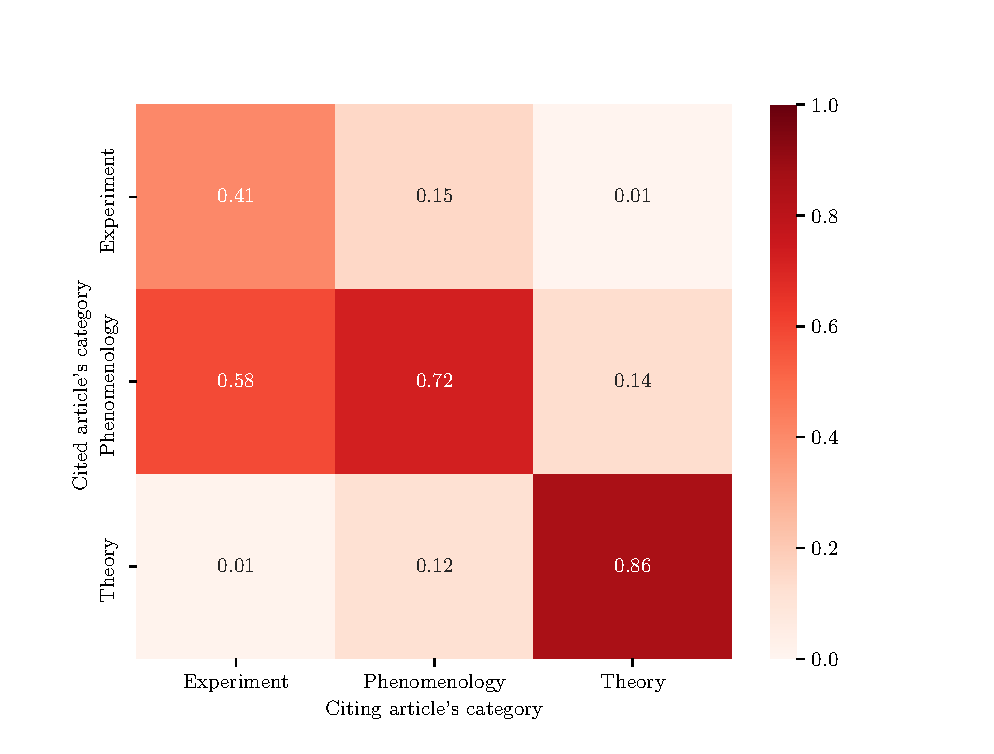
\includegraphics{Fig9.eps}
\caption{\label{fig:tsne}Semantic map extracted from the topic model, after applying a t-SNE transformation. Each dot represents a topic. Each topic is assigned the category, among theory, phenomenology and experiment, that is most associated with it. Correlated topics appear closer to each other. For each category, the density of topics along the x-axis is shown in the lower plot.}
\end{figure}

Although the t-SNE transformation does not yield very stable results, it generally appears (as in this figure) that topics most associated with a given category (e.g. theory) appear closer to each other, such that these three categories explain part of the variance in the semantic space. Second, in this representation, the distinction between phenomenological supersymmetry and theoretical supersymmetry is supported by the emergence of two separate clusters of supersymmetry-related topics.


\section{\label{appendix:phenomenology_centrality}Validity of the citation network for exploring the trading zone}

Below, we support the relevance of the citation network as a means of exploring trading zones between scientific cultures by showing it can be used to recover known facts, in particular i) that theory and experiment in HEP do not communicate directly and ii) that phenomenology channels most exchanges across them.

We build a citation network where each node is one paper of the literature and the edge between nodes $x$ and $y$ is assigned a weight $w_{x,y}=1$ if $x$ cites $y$ and 0 otherwise. From this we can define the amount of citations of papers from the category $i$ to a paper from the category $j$ as: 

\begin{equation}
    \label{eq:cite_matrix}
    n_{ij} = \sum_{x\in i, y\in j} \dfrac{w_{xy}}{(\sum_c \mathds{1}_c(x))(\sum_c \mathds{1}_c(y))} 
\end{equation}

Where $\mathds{1}_c(x)=1$ if $x$ belongs to $c \in \{$Experiment, Phenomenology, Theory$\}$, and 0 otherwise. 
We then normalize $n_{ij}$ by the amount of citations \textit{from} category $i$, thus yielding the normalized matrix $\tilde{n}_{ij}$. By construction, $0\leq \tilde{n}_{ij}\leq 1$ is the effective fraction of references from papers of category $i$ to papers of category $j$. The matrix is built from the citation network between 2001 and 2019. We then verify that $\tilde{n}_{ii}$ is high (papers mostly cite papers from the same category); and that for cross-culture citations ($i\neq j$), $\tilde{n}_{ij} \ll 1$ unless $i$ or $j$ is ``phenomenology''; i.e., ``trading zones'' in the field occur around phenomenology. Evaluating the fraction of citations from papers of a category $i$ that target papers from a category $j$ yields the matrix in Figure \prettyref{fig:cites_matrix}. In this matrix, borrowing the trade metaphor from \citet{Yan2013}, non-diagonal elements represent ``imports'' (references to publications from other subcultures) and diagonal elements measure the ``self-dependence'' of each subculture. The results confirm that most citations occur within categories, emphasizing the relative autonomy of each of these subcultures including phenomenology -- it is less obvious for experimental papers, which are much more scarce then the others, and cannot cite themselves as much. Moreover the results confirm that most trades involve phenomenology: cross-citations between purely theoretical and experimental papers are very rare ($\sim$1\% of their references). Overall, ``theory'' is highly self-reliant.

\begin{figure*}
    \centering
    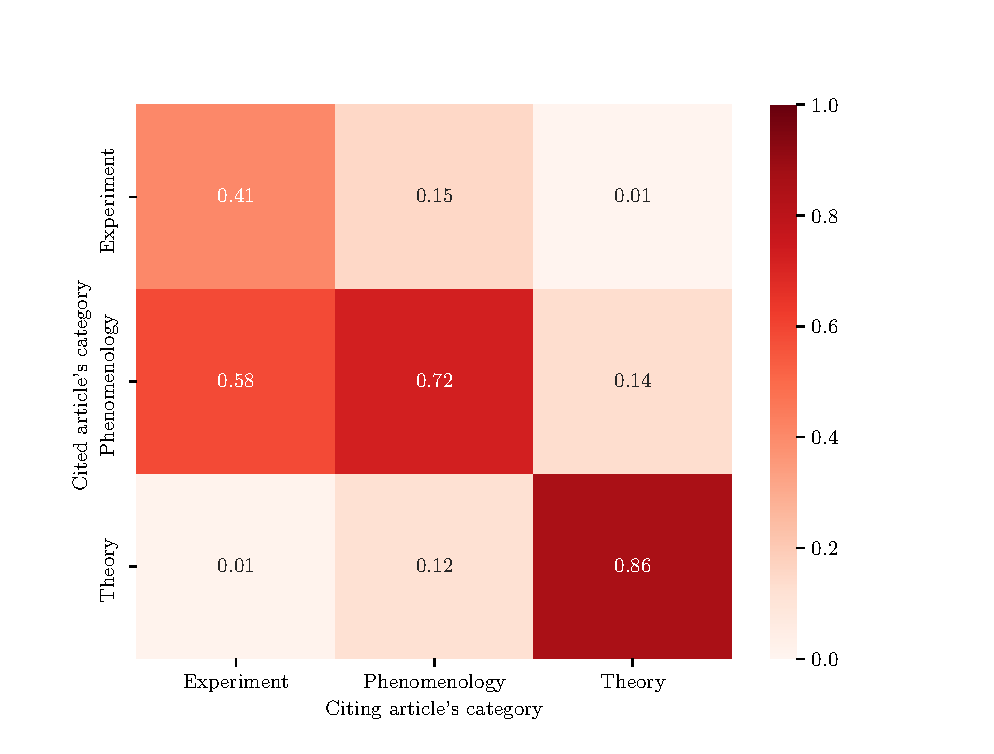
\includegraphics{Fig10.eps}
    \caption{\textbf{Origin of the references (citations) in the \gls{hep} literature}
    Each matrix element $\tilde{n}_{ij}$ represents the fraction of references from the x-axis category (columns) that target papers from the y-axis category (lines). For instance, 41\% of references in experimental papers refer to experimental papers. 15\% of citations from phenomenological papers refer to experimental papers. If these categories were completely hermetic, the matrix would equal the identity matrix, which is not the case.}
    \label{fig:cites_matrix}
\end{figure*}

\printbibliography

\end{document}